%
% 1- The Idea.tex
%
% This LaTeX source file is for section 1- The Idea for
% the Conceptual Clustering Search Algorithm lab module 
% for the TAILS project under Dr. Stephanie August.
%
\section{The Idea}
\subsection{Purpose}
The purpose of this lab is to familiarize the experimenter with machine learning in general and the COBWEB conceptual clustering algorithm specifically. Experimenter will be provided with a visualized simulation tool, which takes in objects defined and inputted by the experimenter and displays the dynamic spanning of the classification based on input.

\subsection{Background}

\subsubsection {Machine Learning}
People are able to learn new things. What exactly does it mean about machine learning?  Arthur Samuel defined machine learning as a \lq\lq{field of study that gives computers the ability to learn without being explicitly programmed}\rq\rq\cite{simon2013too}. In 1997, Tom M. Mitchell gave a more formal definition: \lq\lq{A computer program is said to learn from experience E with respect to some class of tasks T and performance measure P, if its performance at tasks in T, as measured by P, improves with experience E}\rq\rq\cite{mitchell1997machine}. A possible example to explain E, P, T here could be the email spam filtering program. The email program learns from users which emails are marked as spam and which are not. Based on these data, the program learns to filter spam. In this machine learning case, E is watching user mark emails as spam or as not spam, T is classifying emails as spam or as not spam, and P could be the number of emails correctly classified as spam\cite{stanford}.

\subsubsection {Supervised Learning VS Unsupervised Learning}
Based on the desired outcome of the algorithm or the type of input available during training the machine, machine learning usually can be divided into two main types: the predictive or supervised learning approach and the descriptive or unsupervised learning approach\cite{murphy2012machine}. The idea of supervised learning is to teach the program to do something, whereas unsupervised learning is going to let the program learn by itself. 

In supervised learning, the algorithm is given data in which it is told the \lq\lq{correct answer}\rq\rq for each example\cite{stanford}. Classification is probably the most widely used form of supervised learning. One example could be the email spam filtering algorithm mentioned above. Whenever a new email is detected, the algorithm will decide whether it is a spam or not and then put it in the right category the algorithm believes.  

Unlike supervised learning, we are not told what the desired output is for each input in unsupervised learning. We are just given a bunch of data and will discover any interesting structure in the data. So in unsupervised learning, no one tells you which data is what. All the information lie in the input data. What we need to do is to formalize our task as one of density estimation\cite{murphy2012machine}. The most common form of unsupervised learning is clustering.

\subsubsection {Clustering}
Clustering is the process of grouping similar objects together, so that objects within each cluster are similar to each other and from different clusters are dissimilar. According to the types of output, there are partitional clustering, where we partition the objects into disjoint sets; and hierarchical clustering, where we create a nested tree of partitions\cite{murphy2012machine}. A simple example of data clustering is shown in Fig\ref{Fig:clustering}. The input data is clearly distributed in six groups, and those data in the same group have the same label which is the desired output clusters.

\begin{figure}[h!]
    \centering
    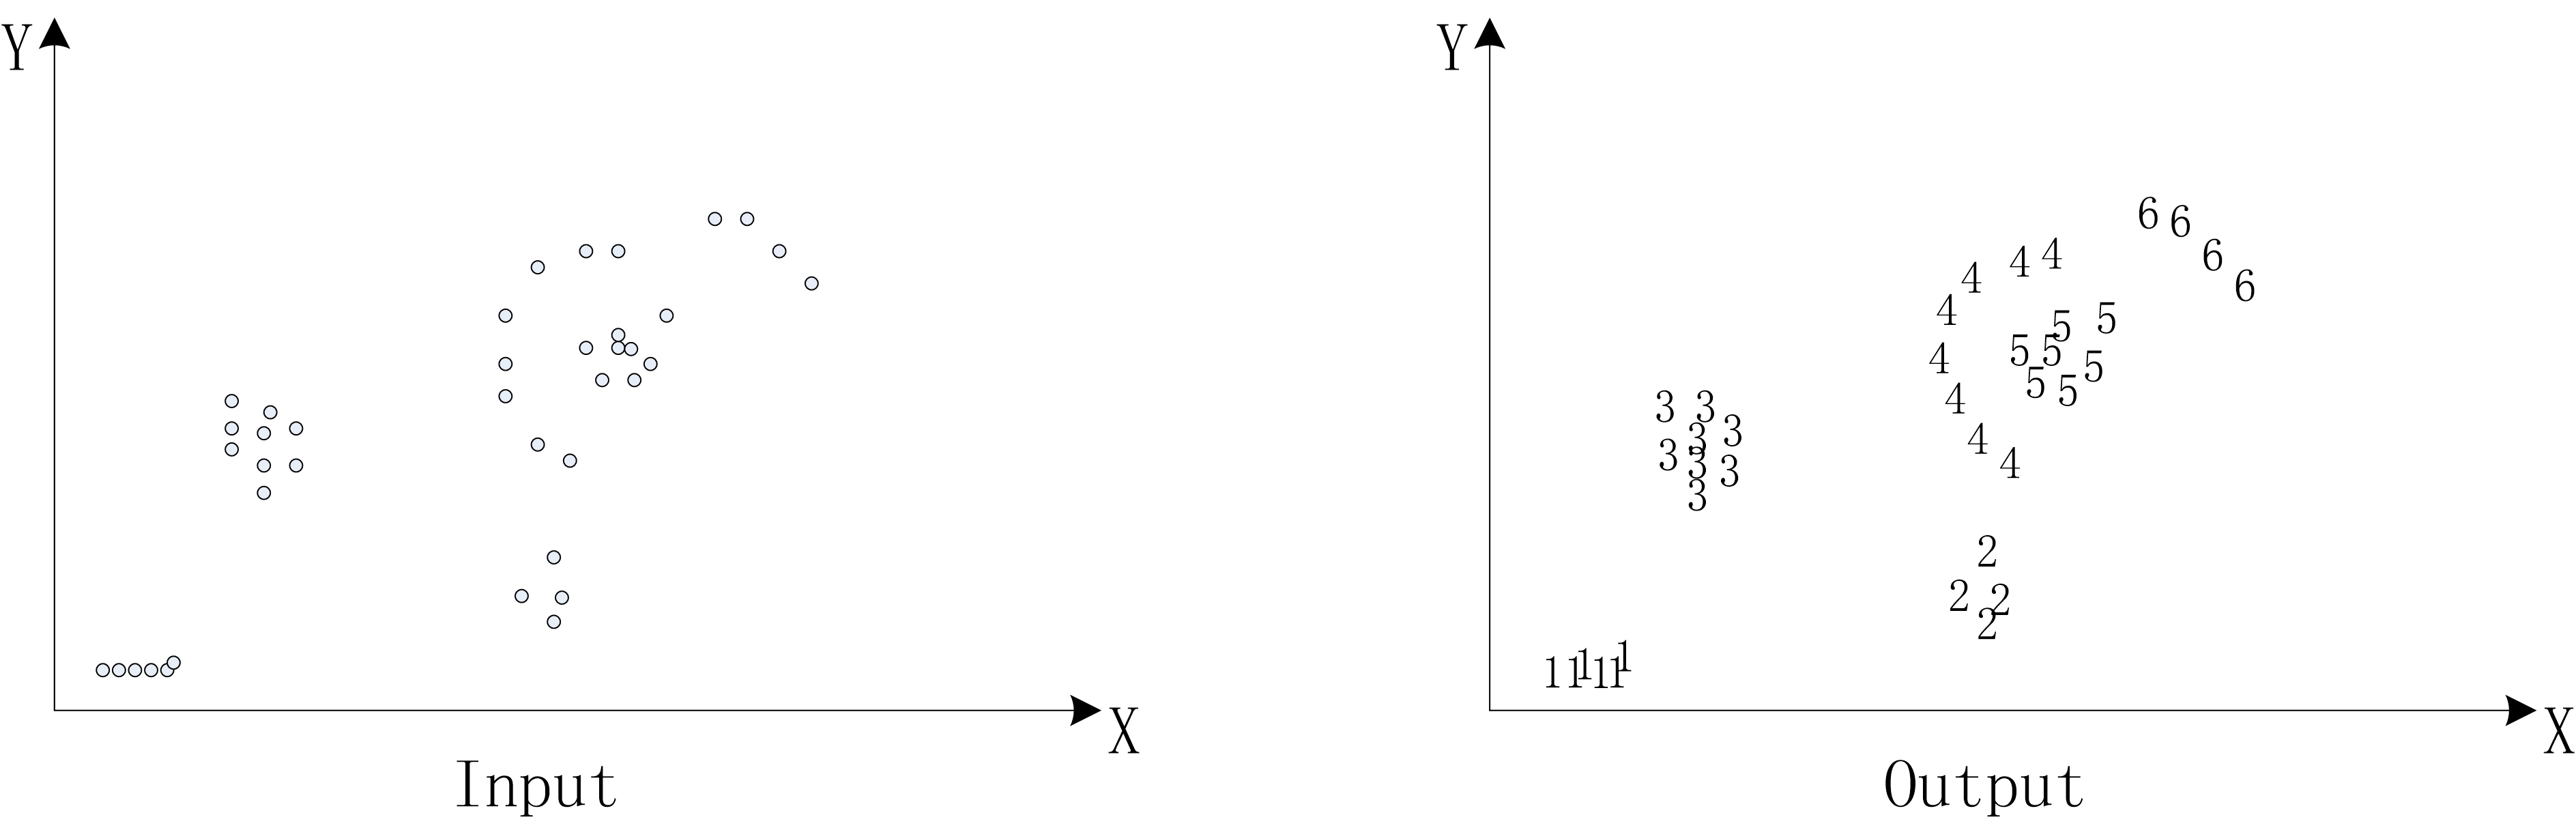
\includegraphics[width=300pt]{../images/clustering.jpg}
    \caption{An example of data clustering}
    \label{Fig:clustering}
\end{figure}
	
Hierarchical clustering algorithms are either top-down or bottom-up. Bottom-up algorithms treat each data as a singleton cluster at the outset and then successively merge (or agglomerate) pairs of clusters until all clusters have been merged into a single cluster that contains all data. Bottom-up hierarchical clustering is therefore called hierarchical agglomerative clustering. Top-down clustering requires a method for splitting a cluster. It proceeds by splitting clusters recursively until individual datum is reached\cite{manning2008introduction}.
% I don't really know what we're going to have the experimenter do yet.
% While performing experiments
% in this lab module, you, the experimenter, will learn how to make slight
% modifications to the basic search algorithm to progress between the different
% search types.
\subsubsection{An incremental conceptual clustering algorithm: COBWEB}

\paragraph{Conceptual Clustering}
Conceptual clustering is closely related to data clustering, however, it is distinguished from ordinary data clustering by generating a concept description for each generated class. In conceptual clustering, it is not only the inherent structure of the data that drives cluster formation, but also the description language which is available to the learner. Thus, a statistically strong grouping in the data may fail to be extracted by the learner if the prevailing concept description language is incapable of describing that particular regularity\cite{wikiconceptualclustering}. 

Conceptual clustering algorithms are generally used in situations where we may not have all the data when we want to start organizing our findings. The main purpose of the conceptual clustering algorithm is to allow for data elements to be organized in relation to each other as more data becomes available.

In most implementations, the description language has been limited to feature conjunction, however, in COBWEB, the feature language is probabilistic.

\paragraph {Incremental Clustering}
Incremental clustering is based on the assumption that it is possible to consider patterns one at a time and assign them to existing clusters. A typical incremental clustering algorithm is described as below\cite{jain1999data}:
\begin{itemize}\setlength{\itemsep}{0.01pt}
\item Assign the first data item to a cluster;
\item Consider the next data item. Either assign this item to one of the existing clusters or assign it to a new cluster. This assignment is done based on some criterion, e.g. the distance between the new item and the existing cluster centroids.
\item Repeat the second step till all the data items are clustered.
\end{itemize}

\paragraph {COBWEB}
The COBWEB conceptual clustering algorithm\cite{fisher1987knowledge} updates the tree (relation of all existing data elements) in accordance with new data that comes in. The tree this algorithm creates is devised in such a way that any \emph{frontier node} is a data element and any \emph{interior node} is a class which is a general representation of all of its children.

% Add picture of classes versus data elements in a tree.
The simplest way of thinking of the COBWEB conceptual clustering algorithm is in terms of a child boy cleaning up his toys (assuming he's only paying attention to the toys he has already organized). Say a child picks up a firetruck first, so he puts the firetruck in its own bin, simply because no bin is in use yet. Then he picks up a bouncy ball. This toy doesn't seem to relate to the firetruck at all, so the child decides to put the bouncy ball in a separate bin from the firetruck. The next toy the child picks up is a racecar. So at this point the child can choose to put the racecar in its own bin, or in the same bin as the firetruck since the racecar and firetruck have a lot in common. The child decides to put the racecar in the same bin as the firetruck because they have enough similarities to share a bin. This is the general concept of the COBWEB conceptual clustering algorithm. As data is brought in, decisions are made.

\subparagraph {Category Utility}
The first step of the COBWEB conceptual clustering algorithm is to determine the best spot for the new data element in the existing tree. That is, to determine which class the new data element fits into best. But one thing to note is that there are situations when the best option is to treat the new data element as its own entity and place it directly under the root node, rather than add it to an existing class.

But once a data element has been added to a class, there may be sub-classes into which it might fit better than the class it is currently assigned to. So in order to determine the best place for a new data element, the algorithm could possibly have to traverse all the way down to a class consisting of \emph{only} frontier nodes.

The next question is, how do we know which spot is \lq\lq{best}\rq\rq for a new element? This is determined by the \emph{categorical utility}\cite{gluck1985information} of adding the new data element to a certain spot in the tree. Category utility can be viewed as a function that rewards traditional virtues held in clustering generally--similarity of objects within the same class and dissimilarity of objects in different classes\cite{fisher1987knowledge}:

\begin{itemize}\setlength{\itemsep}{0.01pt}
\item Intra-class similarity is reflected by conditional probability: $P(A_i=V_{ij}\left|C_k\right.)$, where $A_i$ denotes an attribute, $V_{ij}$ denotes an attribute value, $C_k$ denotes a class. The larger this probability, the greater proportion of class members sharing the value and the more predictable the value is of class members\cite{fisher1987knowledge}.
\item Inter-class similarity is a function of $P(C_k|A_i=V_{ij})$. The larger this probability, the fewer the objects in contrasting classes that share this value and the more predictive the value is of the class\cite{fisher1987knowledge}.
\end{itemize}

Based on the intra-class and inter-class similarity, for a partition $\{C_1, C_2,...,C_n\}$ which is a set of mutually exclusive classes, the following equation $$E_1=\sum_{k=1}^{n}\sum_{i}\sum_{j}P(A_i=V_{ij})P(C_k|A_i=V_{ij})P(A_i=V_{ij}\left|C_k\right.)$$ overall measures the partition quality, where the probability $P(A_i=V_{ij})$ weights the importance of the individual attribute value. $E_1$ indicates that it is more important to increase the class-conditioned predictability and predictiveness of frequently occurring values than for infrequently occurring ones\cite{fisher1987knowledge}.

According to Bayes Rule, $ P(A_i=V_{ij})P(C_k|A_i=V_{ij})=P(C_k)P(A_i=V_{ij}|C_k)$. By substituting to $E_{1}$, we will get:$$E_1=\sum_{k=1}^{n}P(C_k)\sum_i \sum_jP(A_i=V_{ij}\left|C_k\right.)^2$$ which is the ability to correctly guess the attributes of an object in a certain class. 

Finally, category utility is defined by Cluck and Corter as the increase in the expected number of attribute values that can be correctly guessed $P(C_k)\sum_i \sum_jP(A_i=V_{ij}\left|C_k\right.)^2$ over the expected
number of correct guesses without such knowledge $\sum_i \sum_jP(A_i=V_{ij})^2$\cite{fisher1987knowledge}:
\begin{equation*}
\label{eq:cu}
%\text{Category Utility}
CU=\frac{\sum_{k=1}^{n}P(C_k)\left[\sum_i \sum_jP(A_i=V_{ij}\left|C_k\right.)^2-\sum_i \sum_jP(A_i=V_{ij})^2\right]}{n}
\end{equation*}

Here is an example: if a class has 8 green balls and 2 red balls and a different class has 4 green squares and 7 blue squares and the new element is a blue ball, the new blue ball will be placed in the first class according to the category utility since the CU value for this partition is the highest.
\begin{table}[!ht]
\ttabbox{\caption{Table of Classes}}{
\centering
\begin{minipage}{0.45\textwidth}
\begin{tabular}{l l l}\hline
\textbf{ } & \textbf{Class 1} & \textbf{ }\\
\textbf{A1} & \textbf{A2} & \textbf{Number}\\\hline
Green & Ball & 8 \\
Red & Ball & 2 \\\hline
\end{tabular}
\end{minipage}
\hfil
\begin{minipage}{0.45\textwidth}
\begin{tabular}{l l l}\hline
\textbf{ } & \textbf{Class 2} & \textbf{ }\\
\textbf{A1} & \textbf{A2} & \textbf{Number}\\\hline
Green & Square & 4 \\
Blue & Square & 7 \\\hline
\end{tabular}
\label{tab:label}
\end{minipage}}
\end{table}
% Check the above example

By the definition above, we can say in this example, there are two classes $C_1$ and $C_2$ (shown in Table \ref{tab:label}), and two attributes \emph{color} and \emph{shape} with five attribute values which are: $$A_1=\{\text{color}|V_{11}=\text{Green},V_{12}=\text{Red}, V_{13}=\text{Blue}\}$$$$A_2=\{\text{shape}|V_{21}=\text{Ball}, V_{22}=\text{Square}\}$$

First, if we place the new element \{Blue Ball\} in Class 1(shown in Table \ref{tab:label2}), we can calculate CU for the current partition. The probability for $C_1$ is $$P(C_1)=\frac{8+2+1}{8+2+1+4+7}=0.5$$ and the probability for $C_2$ is $$P(C_2)=\frac{4+7}{8+2+1+4+7}=0.5$$ 
The expected number of attribute values that can be correctly guessed given $C_1$ is: 
\begin{equation*}
\begin{aligned}
&\sum_{i=1}^{2} \sum_{j=1}^{3}P(A_i =V_{ij}\left|C_1\right.)^2\\
=&(\frac{8}{8+2+1})^2+(\frac{2}{8+2+1})^2+(\frac{1}{8+2+1})^2+(\frac{8+2+1}{8+2+1})^2+0\\
=&1.5702
\end{aligned}
\end{equation*} % % % too long to put in one line
and the expected number of attribute values that can be correctly guessed given $C_2$ is: $$\sum_{i=1}^{2} \sum_{j=1}^{3}P(A_i=V_{ij}\left|C_2\right.)^2=(\frac{4}{4+7})^2+0+(\frac{7}{4+7})^2+0+(\frac{4+7}{4+7})^2=1.5372$$
%\begin{equation*}
%\begin{aligned}
%\end{aligned}
%\end{equation*} 
The expected number of attribute values that can be correctly guessed without any category knowledge is: $$\sum_{i=1}^{2} \sum_{j=1}^{3}P(A_i=V_{ij})^2=(\frac{8+4}{8+2+1+4+7})^2+(\frac{2}{22})^2+(\frac{1+7}{22})^2+(\frac{8+2+1}{22})^2+(\frac{4+7}{22})^2=0.9380$$ 
Thus, we can get CU for adding the new element to the Class 1: $$CU_1=\frac{0.5\times(1.5702-0.9380)+0.5\times(1.5372-0.9380)}{2}=0.30785$$

\begin{table}[!ht]
\ttabbox{\caption{Table of Classes by adding the new element in $C_1$}}{
\centering
\begin{minipage}{0.45\textwidth}
\begin{tabular}{l l l}\hline
\textbf{ } & \textbf{$C_1$} & \textbf{ }\\\hline
\textbf{A1} & \textbf{A2} & \textbf{Number}\\
\hline
Green & Ball & 8 \\
Red & Ball & 2 \\
Blue & Ball & 1\\\hline
\end{tabular}
\end{minipage}
\hfil
\begin{minipage}{0.45\textwidth}
\begin{tabular}{l l l}\hline
\textbf{ } & \textbf{$C_2$} & \textbf{ }\\\hline
\textbf{A1} & \textbf{A2} & \textbf{Number}\\\hline
Green & Square & 4 \\
Blue & Square & 7 \\\hline
\end{tabular}
\label{tab:label2}
\end{minipage}}
\end{table}

Second, in the same manner, we can also get CU for adding the new element to the Class 2(shown in Table \ref{tab:label3}), which is: $$CU_2=\frac{\frac{10}{22}\times(1.68-0.9380)+\frac{12}{22}\times(1.4028-0.9380)}{2}=0.2954$$

\begin{table}[!ht]
\ttabbox{\caption{Table of Classes by adding the new element in $C_2$}}
{
\centering
\begin{minipage}{0.45\textwidth}
\begin{tabular}{l l l}\hline
\textbf{ } & \textbf{$C_1$} & \textbf{ }\\\hline
\textbf{A1} & \textbf{A2} & \textbf{Number}\\
\hline
Green & Ball & 8 \\
Red & Ball & 2 \\
\hline
\end{tabular}
\end{minipage}
\hfil
\begin{minipage}{0.45\textwidth}
\begin{tabular}{l l l}\hline
\textbf{ } & \textbf{$C_2$} & \textbf{ }\\\hline
\textbf{A1} & \textbf{A2} & \textbf{Number}\\\hline
Green & Square & 4 \\
Blue & Square & 7 \\
Blue & Ball & 1\\\hline
\end{tabular}
\label{tab:label3}
\end{minipage}}
\end{table}

Last, besides the possibility that placing the new element in an existing class, there is a chance for the new element generate a new class by itself. In the same manner, we can further calculate CU for generating a new class for the new element(shown in Table \ref{tab:label4}), which is $$CU_3=\frac{\frac{10}{22}\times(1.68-0.9380)+\frac{11}{22}\times(1.5372-0.9380)+\frac{1}{22}\times(2-0.9380)}{3}=0.2284$$ 
\begin{table}[!ht]
\ttabbox{\caption{Table of Classes by generating a new class with the new element}}
{
\centering
\begin{minipage}{0.35\textwidth}
\begin{tabular}{l l l}\hline
\textbf{ } & \textbf{$C_1$} & \textbf{ }\\\hline
\textbf{A1} & \textbf{A2} & \textbf{Number}\\
\hline
Green & Ball & 8 \\
Red & Ball & 2 \\
\hline
\end{tabular}
\end{minipage}
\hfil
\begin{minipage}{0.35\textwidth}
\begin{tabular}{l l l}\hline
\textbf{ } & \textbf{$C_2$} & \textbf{ }\\\hline
\textbf{A1} & \textbf{A2} & \textbf{Number}\\\hline
Green & Square & 4 \\
Blue & Square & 7 \\
\hline
\end{tabular}
\end{minipage}
\hfil
\begin{minipage}{0.35\textwidth}
\begin{tabular}{l l l}\hline
\textbf{ } & \textbf{$C_3$} & \textbf{ }\\\hline
\textbf{A1} & \textbf{A2} & \textbf{Number}\\\hline
Blue & Ball & 1\\\hline
\end{tabular}
\label{tab:label4}
\end{minipage}}
\end{table}

\subparagraph {COBWEB Operations}
The COBWEB algorithm constructs a classification tree incrementally by inserting the objects into the tree one by one. When inserting an new object into the classification tree, the COBWEB algorithm descend the tree along a path of \lq\lq{best matching nodes}\rq\rq\cite{luger2011artificial} and performing one of the following operations at each level\cite{fisher1987knowledge}:
\begin{itemize}\setlength{\itemsep}{0.01pt}
\item Create the new object as a new class
\item Add the new object to an existing class with the highest CU
\item Merge two classes into a single class, or
\item Split a class into several classes
\end{itemize}

In the following, we will demonstrate each operation by taking the example of animal descriptions from the reference\cite{fisher1987knowledge}. 
\begin{table}[!ht]
\ttabbox{\caption{Table of Animal Descriptions}}
{
\centering
\begin{tabular}{l l l l l}\hline
\textbf{Name} & \textbf{Body Cover} & \textbf{Heart Chamber} & \textbf{Body Temp} & \textbf{Fertilization}\\\hline
\textbf{Mammal} & \textbf{Hair} & \textbf{4} & \textbf{Regulated} & \textbf{Internal}\\
\textbf{Bird} & \textbf{Feathers} & \textbf{4} & \textbf{Regulated} & \textbf{Internal}\\
\textbf{Reptile} & \textbf{Cornified-skin} & \textbf{Imperfect 4} & \textbf{Unregulated} & \textbf{Internal}\\
\textbf{Amphibian} & \textbf{Moist-skin} & \textbf{3} & \textbf{Unregulated} & \textbf{External}\\
\textbf{Fish} & \textbf{Scales} & \textbf{2} & \textbf{Unregulated} & \textbf{External}\\
\hline
\end{tabular}
\label{tab:animal}}
\end{table}

Suppose the current classification tree has been built by \lq{\emph{fish}}\rq and  \lq{\emph{amphibian}}\rq from Table\ref{tab:animal}. The tree is shown in Figure\ref{Fig:animaltree}. Listed with each box(node) are the probability of the class and the conditional probabilities of attribute values given the current class.
\begin{figure}[!ht]
    \centering
    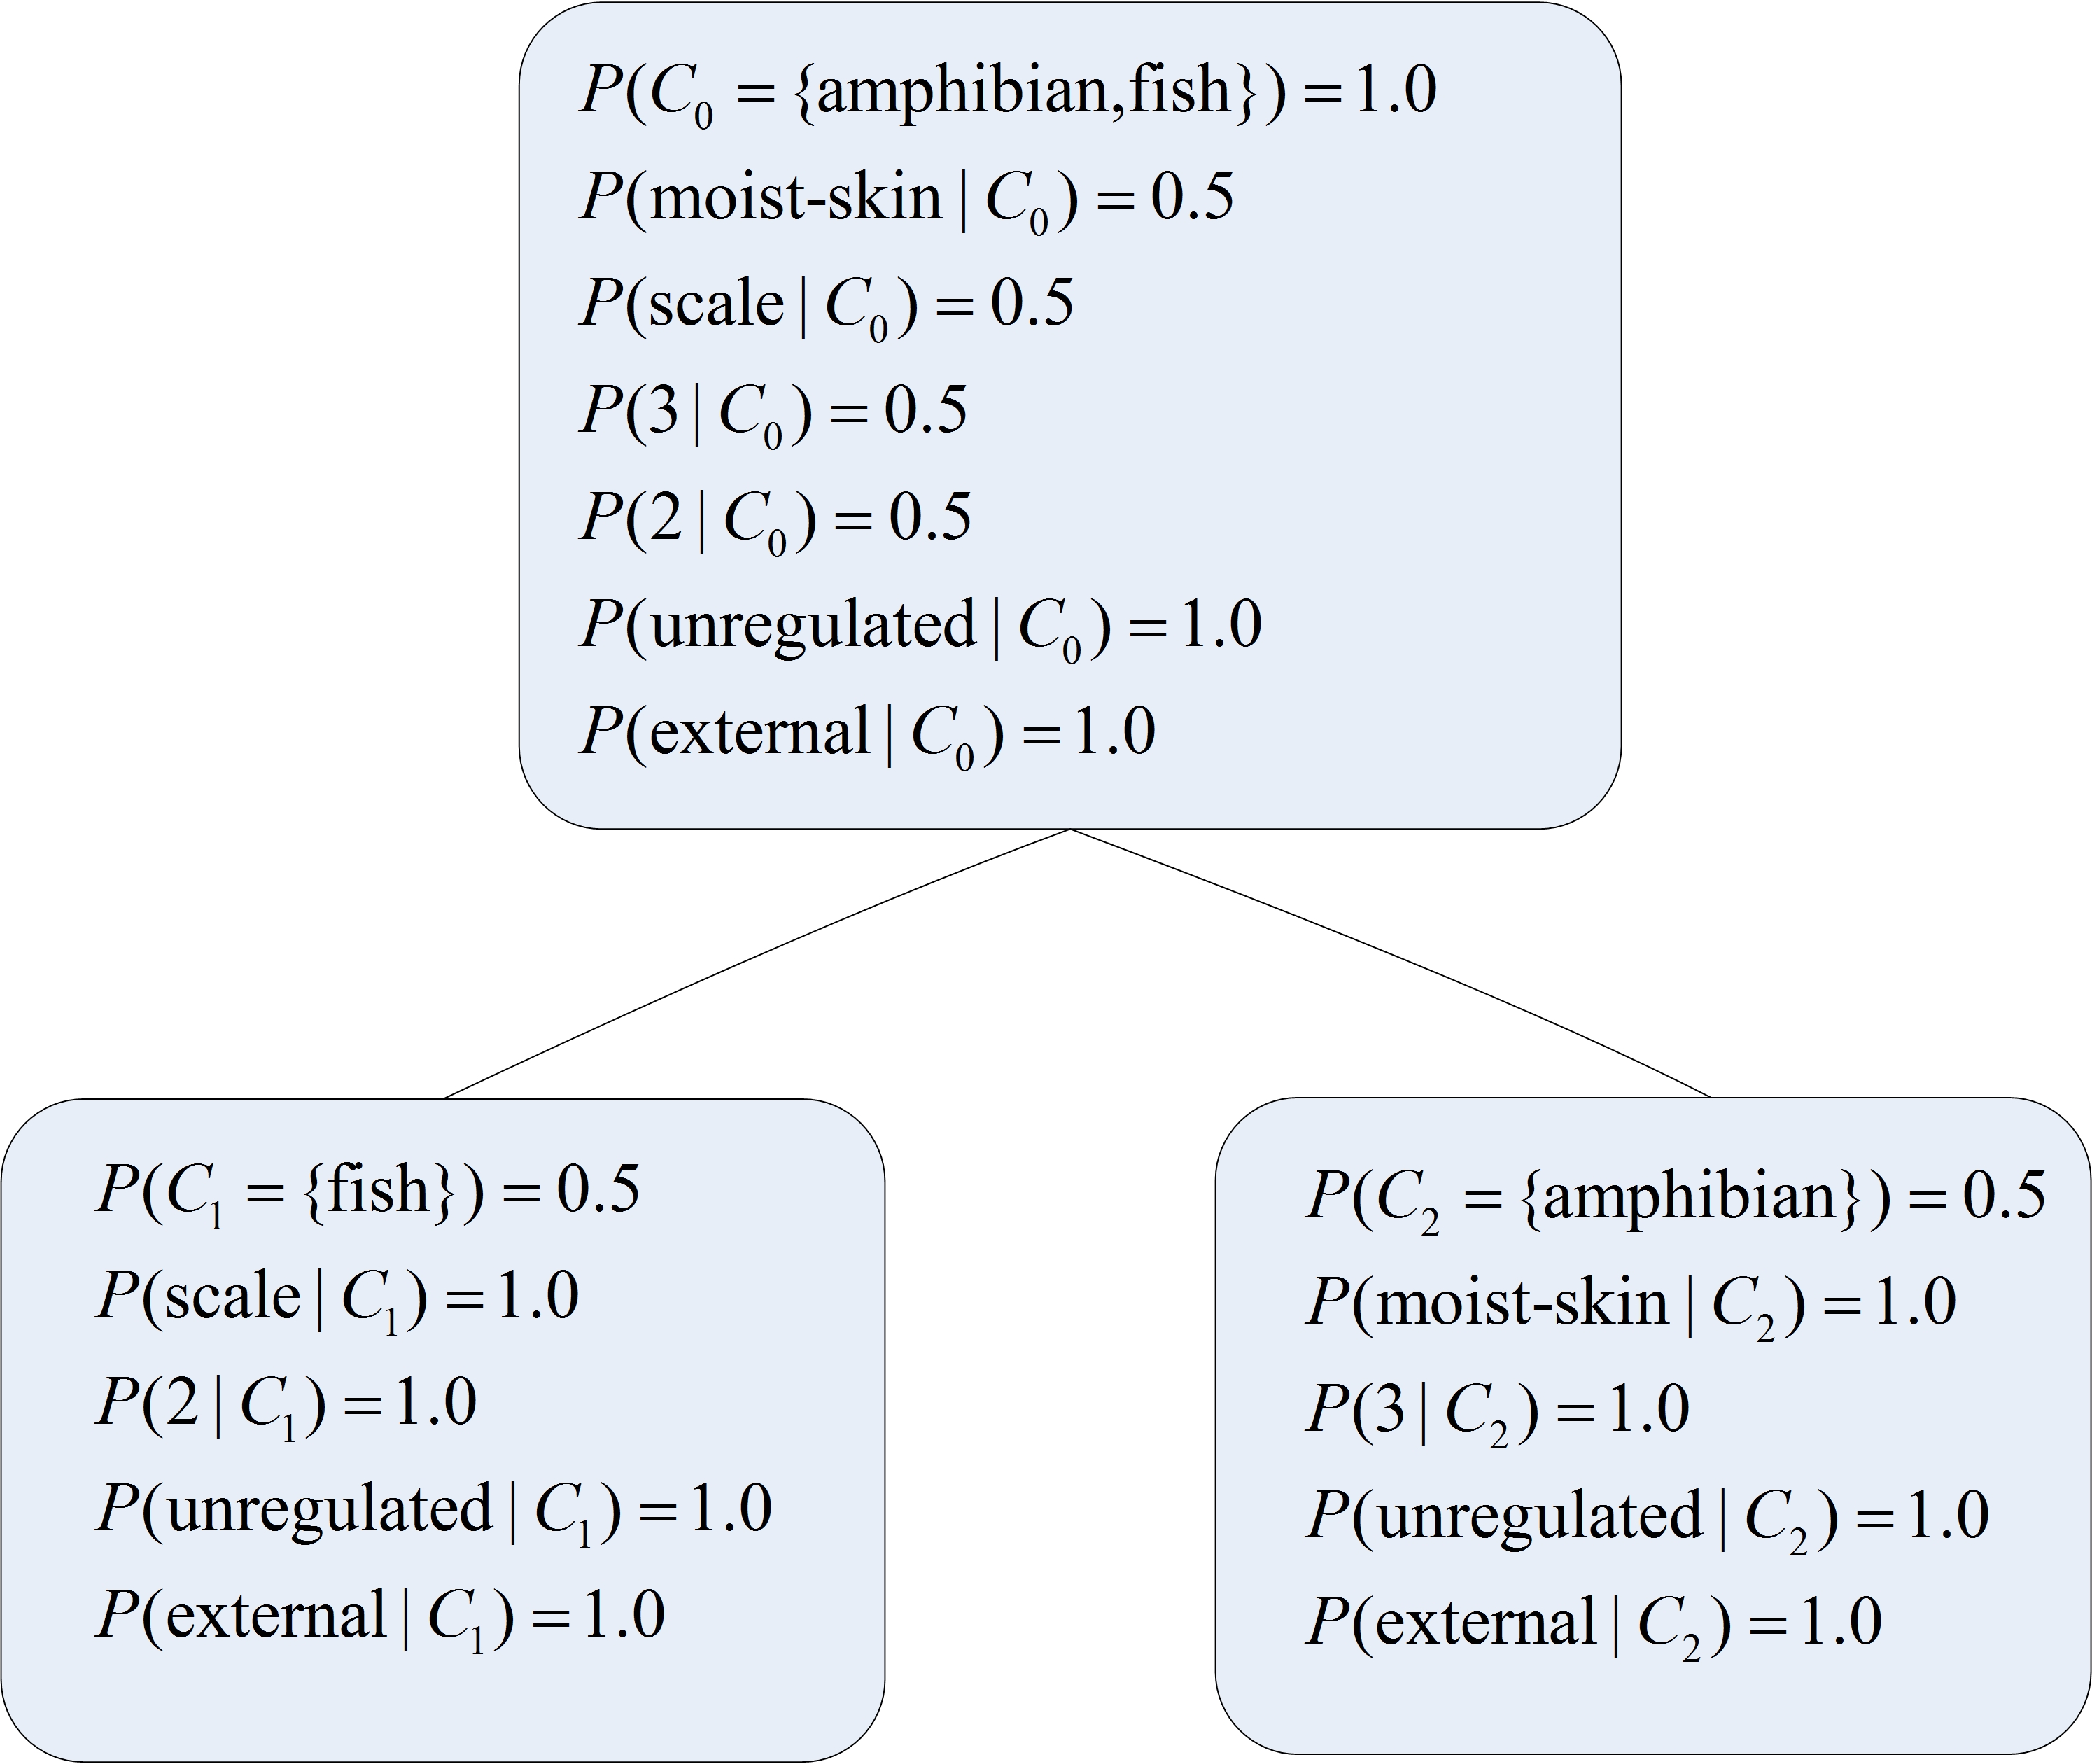
\includegraphics[width=200pt]{../images/animaltree.jpg}
    \caption{Classification tree built by \emph{fish} and \emph{amphibian}}
    \label{Fig:animaltree}
\end{figure}

\textbf{\emph{Creating the new object as a new class}} If the new element \lq{\emph{mammal}}\rq comes, by calculating category utility for classifying \lq{\emph{mammal}}\rq with the existing class \lq{\emph{fish}}\rq, CU for classifying \lq{\emph{mammal}}\rq with the other existing class \lq{\emph{amphibian}}\rq, and CU for creating a new class by \lq{\emph{mammal}}\rq only, we will know where we should put the new element. It turns out that creating a new singleton class with \lq{\emph{mammal}}\rq yields a better partition than adding the element to either of the existing classes. Correspondingly, the tree will transit from the above form to the Figure \ref{Fig:animaltree_create}.
\begin{figure}[!ht]
    \centering
    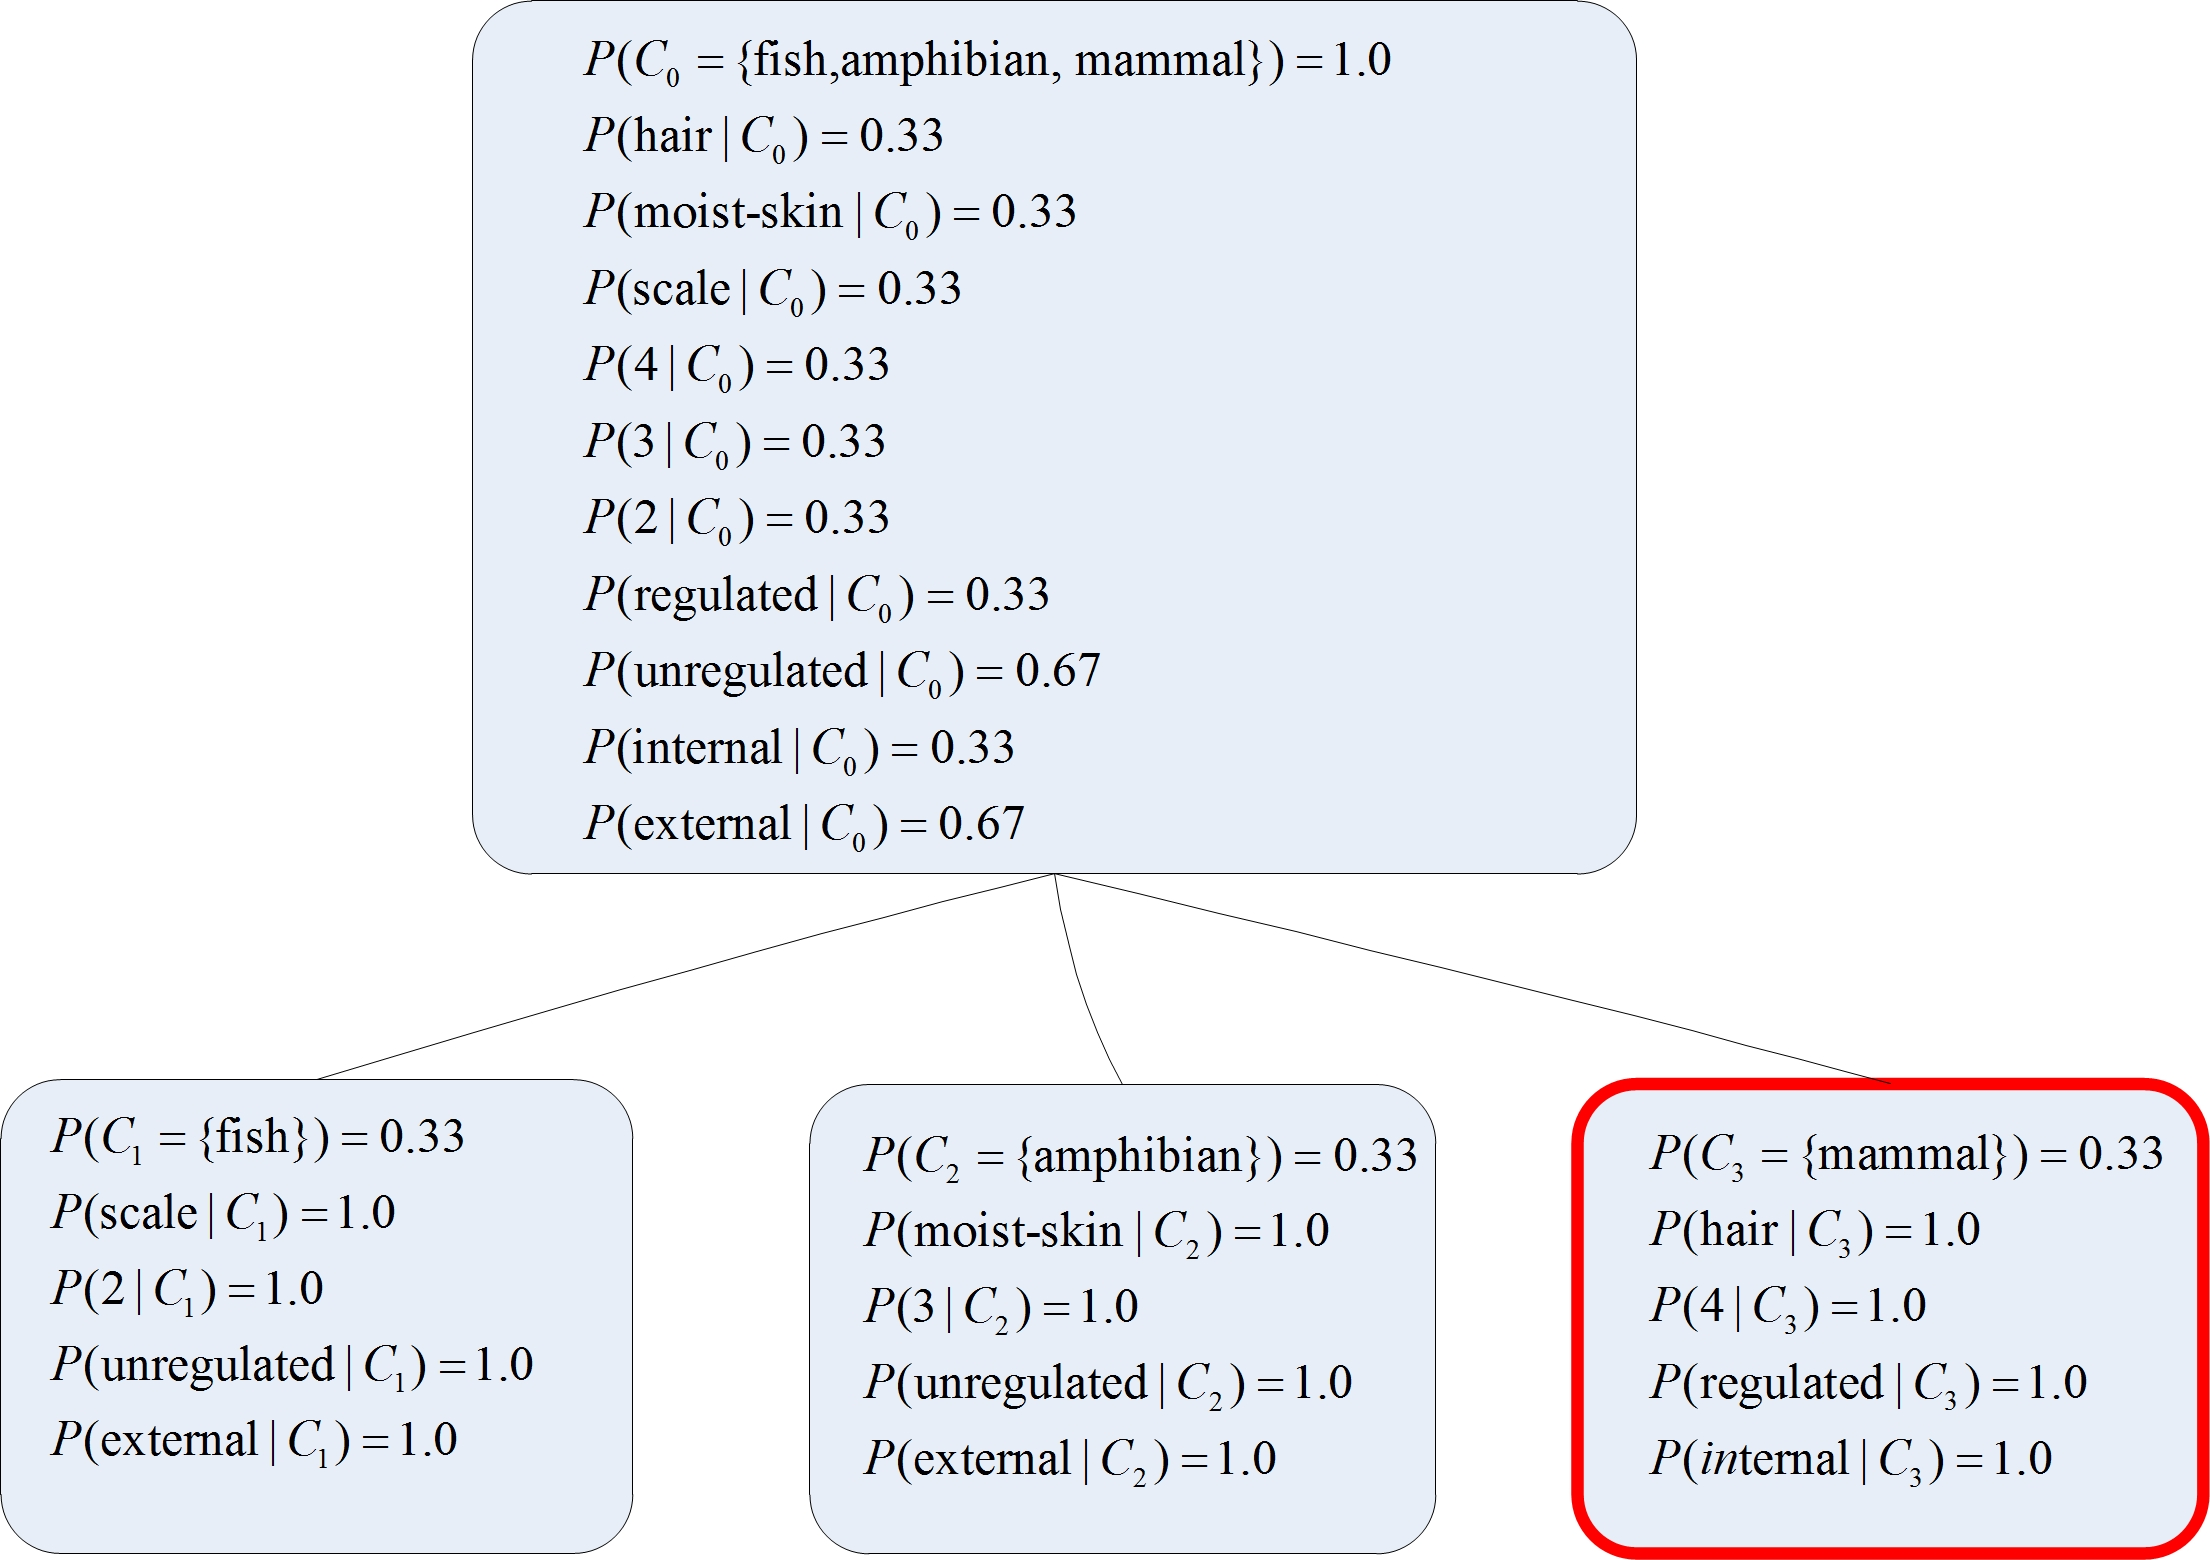
\includegraphics[width=300pt]{../images/animaltree_create.jpg}
    \caption{Adding '\emph{mammal}' to the existing classification tree}
    \label{Fig:animaltree_create}
\end{figure}

\textbf{\emph{Adding the new object to an existing class with the highest CU}} Next, if another new element \lq{\emph{bird}}\rq comes, based on CU, it's easy to know the new element \lq{\emph{bird}}\rq should be added to the existing class \lq{\emph{mammal}}\rq. Since the node \lq{\emph{mammal}}\rq in Figure\ref{Fig:animaltree_create} is a leaf, incorporation of \lq{\emph{bird}}\rq involves expanding the leaf to accommodate the new element \lq{\emph{bird}}\rq, as well as the previously classified one \lq{\emph{mammal}}\rq. The classification tree after \lq{\emph{bird}}\rq is added is shown in Figure\ref{Fig:animaltree_add}.
\begin{figure}[!ht]
    \centering
    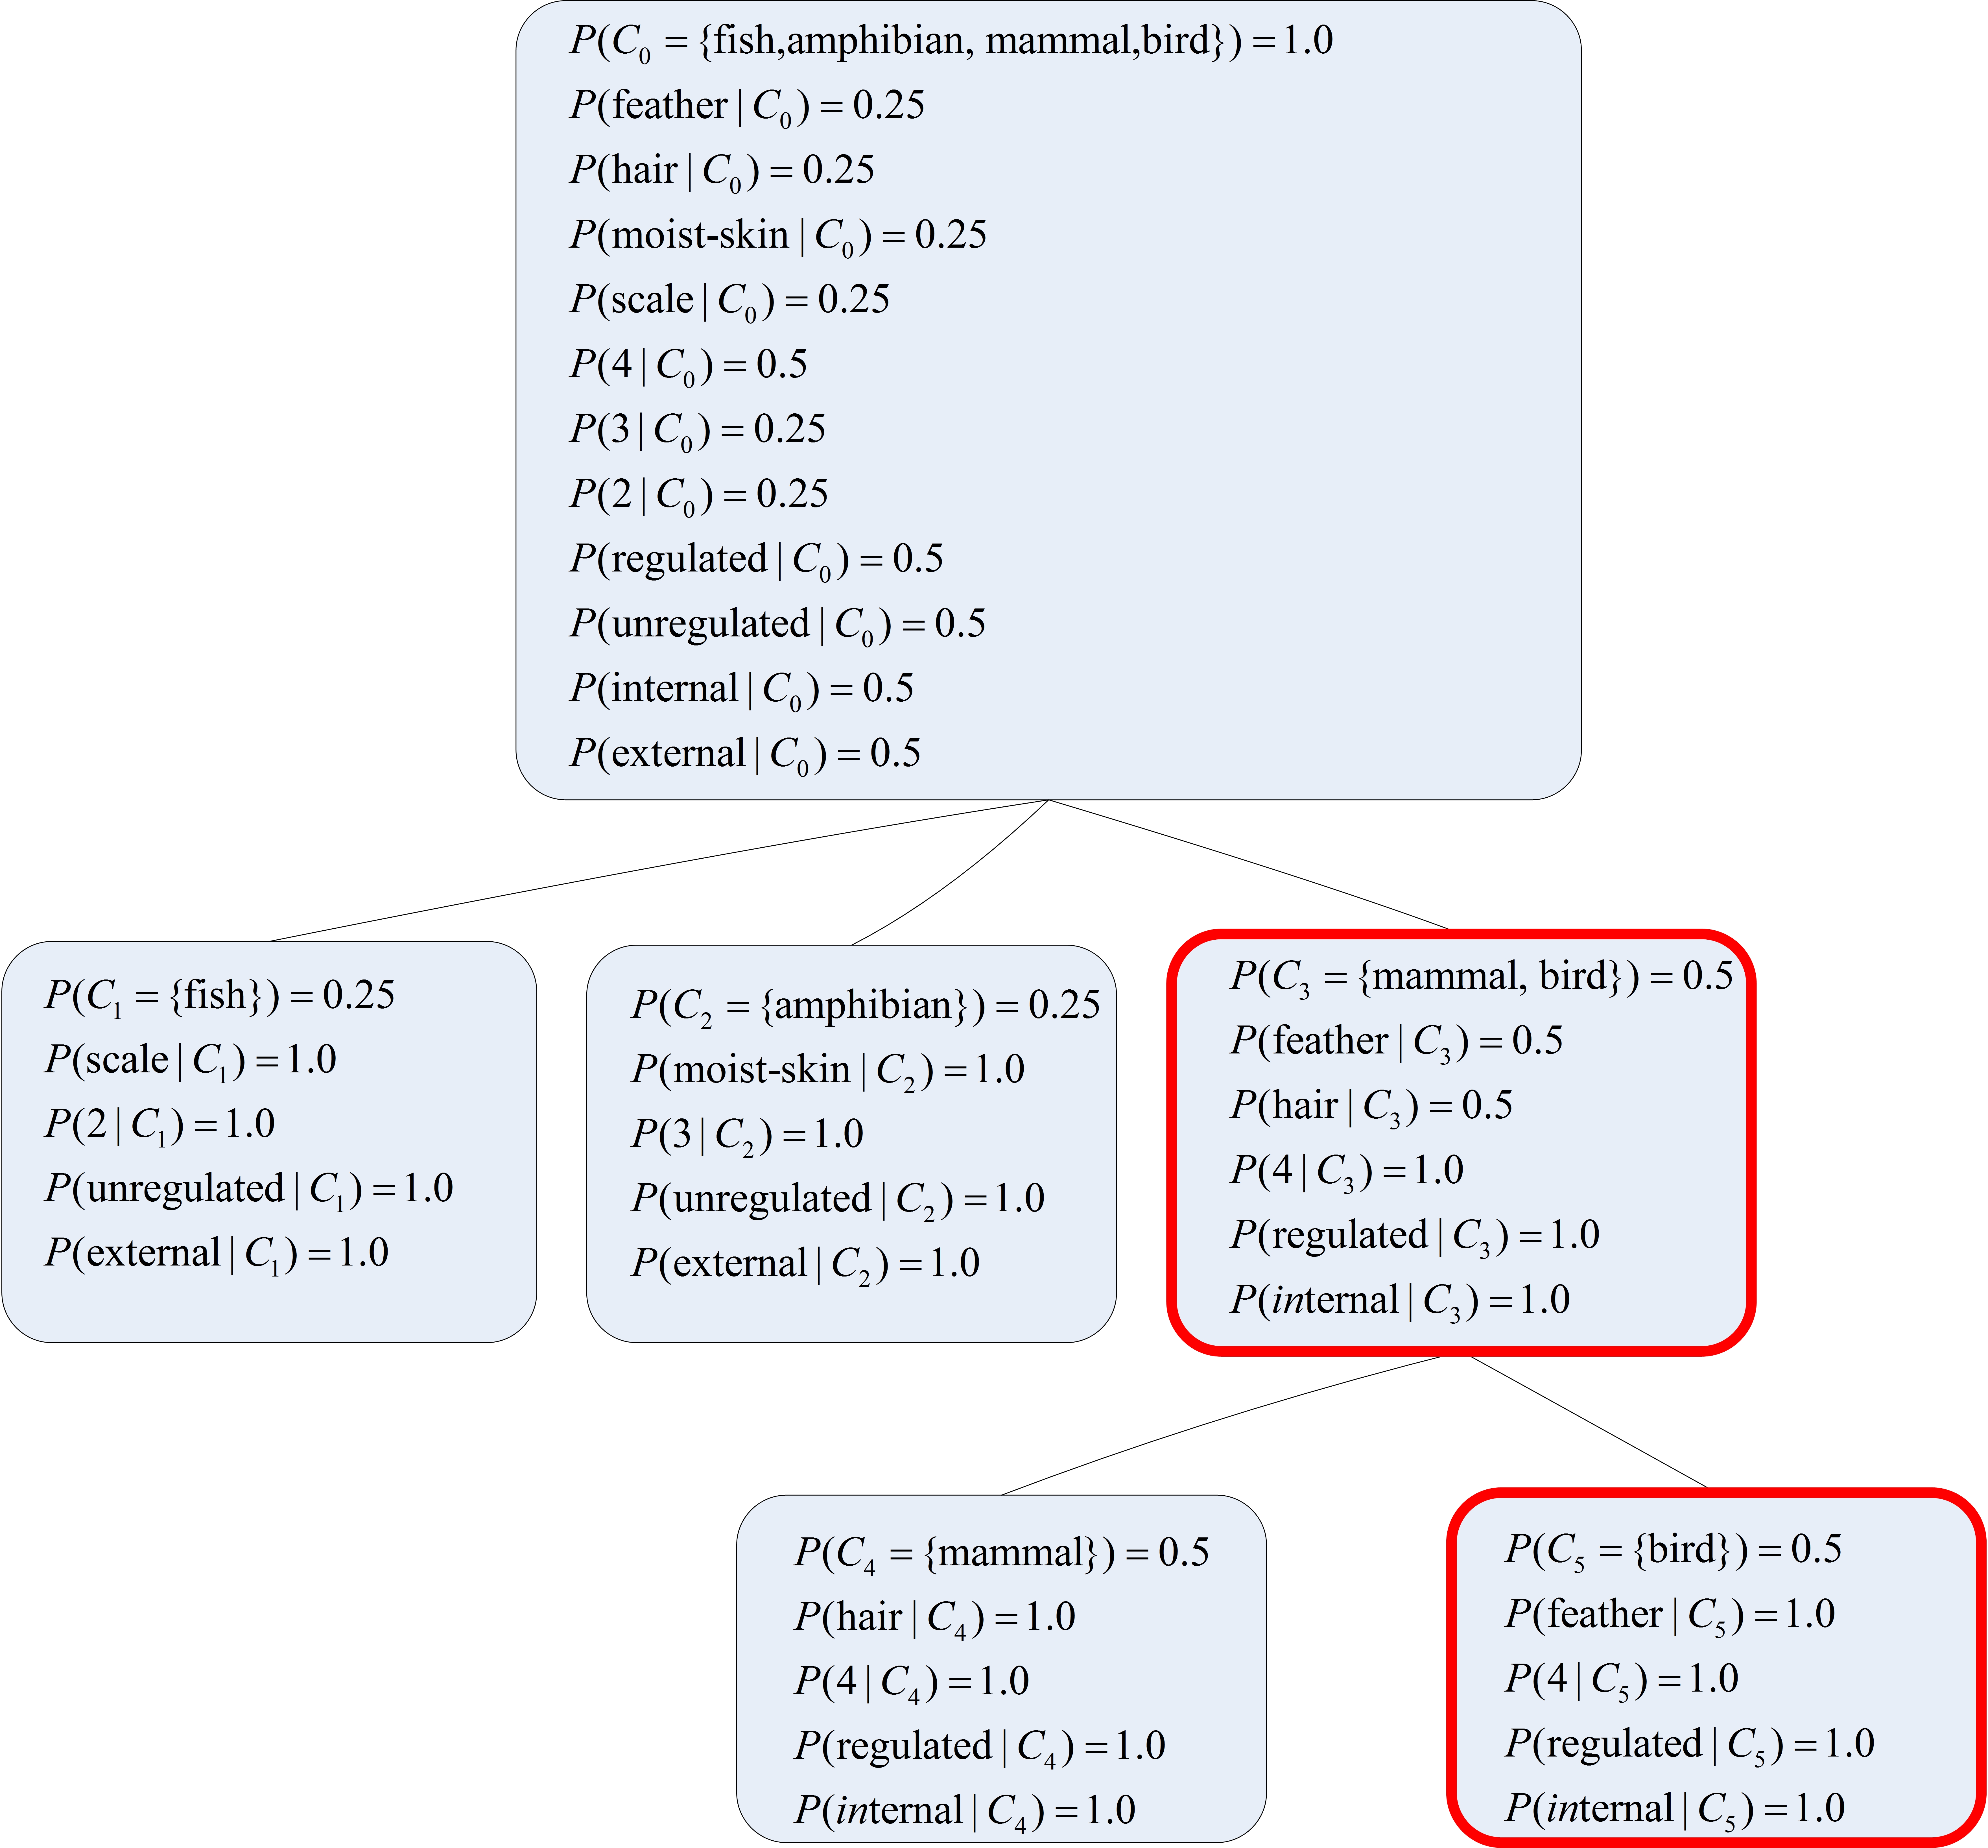
\includegraphics[width=300pt]{../images/animaltree_add.jpg}
    \caption{Adding \lq{\emph{bird}}\rq to the existing classification tree}
    \label{Fig:animaltree_add}
\end{figure}

While the two operations, creating the new object as a new class and adding the new object to an existing class, are effective in many cases, by themselves they are very sensitive to the ordering of initial input. To guard against the effects of initially skewed data, COBWEB includes operations for node merging and splitting. When adding a new object, only the two classes with best CU are considered for merging\cite{fisher1987knowledge}. 

\textbf{\emph{Merging two classes into a single class}} Then, if another element \lq{\emph{fish}}\rq comes, classes $C_1$ and $C_2$ in the Figure \ref{Fig:animaltree_add} are identified as the best and second best hosts for the new element \lq{\emph{fish}}\rq. Merging $C_1$, $C_2$ and the new element \lq{\emph{fish}}\rq results in a partition superior to that obtained by incorporating the new element in the best host $C_1$. The classification tree spanned from Figure \ref{Fig:animaltree_add} is shown in the Figure \ref{Fig:animaltree_merge}.
\begin{figure}[!ht]
    \centering
    \includegraphics[width=300pt]{../images/animaltree_merge.jpg}
    \caption{Adding \lq{\emph{fish}}\rq to the existing classification tree}
    \label{Fig:animaltree_merge}
\end{figure}

\textbf{\emph{Splitting a class into several classes}} Splitting is the inverse operation of merging. Splitting is considered only for the children of the best host among the existing categories. A node of a partition (of n nodes) may be deleted and its children promoted, resulting in a partition of n + m - 1 nodes, where the deleted node had m children\cite{fisher1987knowledge}. An example of splitting is shown in Figure\ref{Fig:split}. 

\begin{figure}[!ht]
    \centering
    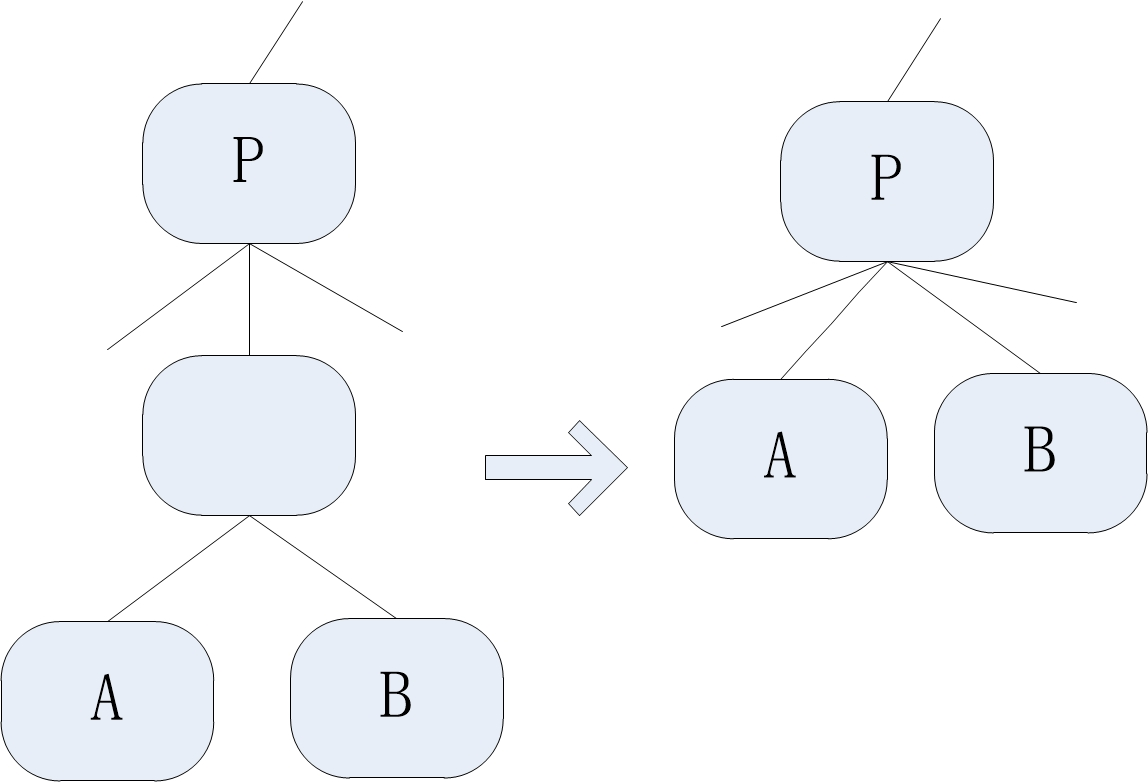
\includegraphics[width=200pt]{../images/split.jpg}
    \caption{An example of node splitting}
    \label{Fig:split}
\end{figure}

\subparagraph {COBWEB Algorithm}
We have detailed the evaluation measure of COBWEB--category utility, and the four operations involved in COBWEB algorithm. The structure of COBWEB algorithm can be summarized as:
\begin{itemize}\setlength{\itemsep}{0.01pt}
\item Tentatively add to each existing portion
\item Calculate CU of each
\item Calculate CU for adding the new object directly to the root
\item Add the new object to the child of the root with the highest CU
\item As with all hill-climbing, presentation order determines initial tree structure
\item MERGE and SPLIT operators minimize the effect of input ordering, and improve partition quality.
\end{itemize}


